%% This is file `elsarticle-template-1a-num.tex',
%%
%% Copyright 2009 Elsevier Ltd
%%
%% This file is part of the 'Elsarticle Bundle'.
%% ---------------------------------------------
%%
%% It may be distributed under the conditions of the LaTeX Project Public
%% License, either version 1.2 of this license or (at your option) any
%% later version.  The latest version of this license is in
%%    http://www.latex-project.org/lppl.txt
%% and version 1.2 or later is part of all distributions of LaTeX
%% version 1999/12/01 or later.
%%
%% The list of all files belonging to the 'Elsarticle Bundle' is
%% given in the file `manifest.txt'.
%%
%% Template article for Elsevier's document class `elsarticle'
%% with numbered style bibliographic references
%%
%% $Id: elsarticle-template-1a-num.tex 151 2009-10-08 05:18:25Z rishi $
%% $URL: http://lenova.river-valley.com/svn/elsbst/trunk/elsarticle-template-1a-num.tex $
%%
\documentclass[preprint,12pt]{elsarticle}

%% Use the option review to obtain double line spacing
%% \documentclass[preprint,review,12pt]{elsarticle}

%% Use the options 1p,twocolumn; 3p; 3p,twocolumn; 5p; or 5p,twocolumn
%% for a journal layout:
%% \documentclass[final,1p,times]{elsarticle}
%% \documentclass[final,1p,times,twocolumn]{elsarticle}
%% \documentclass[final,3p,times]{elsarticle}
%% \documentclass[final,3p,times,twocolumn]{elsarticle}
%% \documentclass[final,5p,times]{elsarticle}
%% \documentclass[final,5p,times,twocolumn]{elsarticle}

%% if you use PostScript figures in your article
%% use the graphics package for simple commands
%% \usepackage{graphics}
%% or use the graphicx package for more complicated commands
%% \usepackage{graphicx}
%% or use the epsfig package if you prefer to use the old commands
%% \usepackage{epsfig}

%% The amssymb package provides various useful mathematical symbols
\usepackage{amssymb}
%% The amsthm package provides extended theorem environments
%% \usepackage{amsthm}

%% The lineno packages adds line numbers. Start line numbering with
%% \begin{linenumbers}, end it with \end{linenumbers}. Or switch it on
%% for the whole article with \linenumbers after \end{frontmatter}.
%% \usepackage{lineno}

%% natbib.sty is loaded by default. However, natbib options can be
%% provided with \biboptions{...} command. Following options are
%% valid:

%%   round  -  round parentheses are used (default)
%%   square -  square brackets are used   [option]
%%   curly  -  curly braces are used      {option}
%%   angle  -  angle brackets are used    <option>
%%   semicolon  -  multiple citations separated by semi-colon
%%   colon  - same as semicolon, an earlier confusion
%%   comma  -  separated by comma
%%   numbers-  selects numerical citations
%%   super  -  numerical citations as superscripts
%%   sort   -  sorts multiple citations according to order in ref. list
%%   sort&compress   -  like sort, but also compresses numerical citations
%%   compress - compresses without sorting
%%
%% \biboptions{comma,round}

% \biboptions{}

%%%%%%%%%%%%%%%%%%%%%%%%%%%%%%%%%
% our packages and definitions: %
%%%%%%%%%%%%%%%%%%%%%%%%%%%%%%%%%
\usepackage{url} 
\usepackage{color}
% \usepackage{dsfont}
\usepackage{booktabs}
\usepackage{amsmath}

\newcommand{\TODO}[1]{{\color{red}TODO: #1}}
\newcommand{\TODON}[1]{{\color{blue}TODO: #1}}
\newcommand{\COMMENTD}[1]{{\color{green}Dimo: #1}}
\newcommand{\COMMENTN}[1]{{\color{green}Nora: #1}}


\journal{DAM}

\begin{document}

\begin{frontmatter}

%% Title, authors and addresses

%% use the tnoteref command within \title for footnotes;
%% use the tnotetext command for the associated footnote;
%% use the fnref command within \author or \address for footnotes;
%% use the fntext command for the associated footnote;
%% use the corref command within \author for corresponding author footnotes;
%% use the cortext command for the associated footnote;
%% use the ead command for the email address,
%% and the form \ead[url] for the home page:
%%
%% \title{Title\tnoteref{label1}}
%% \tnotetext[label1]{}
%% \author{Name\corref{cor1}\fnref{label2}}
%% \ead{email address}
%% \ead[url]{home page}
%% \fntext[label2]{}
%% \cortext[cor1]{}
%% \address{Address\fnref{label3}}
%% \fntext[label3]{}

\title{An Evolutionary Algorithm for the Multiobjective Risk-Equity Constrained Routing Problem}

%% use optional labels to link authors explicitly to addresses:
%% \author[label1,label2]{<author name>}
%% \address[label1]{<address>}
%% \address[label2]{<address>}

\author{Dimo Brockhoff}
\address{INRIA Lille - Nord Europe, DOLPHIN team, 59650 Villeneuve d'Ascq, France\\
{\upshape \url{dimo.brockhoff@inria.fr}}}

\author{Nora Touati-Moungla}
\address{Laboratoire d'Informatique, \'{E}cole Polytechnique, 91128 Palaiseau Cedex, France\\
{\upshape \url{touati@lix.polytechnique.fr}}}



\begin{abstract}
tbw
\end{abstract}

\begin{keyword}
Evolutionary multiobjective optimization, Transportation of hazardous materials, Risk equity, Shortest Paths. 
\end{keyword}

\end{frontmatter}


%%%%%%%%%%%%%%%%%%%%%%%%%%%%%%%%%%%%%%%%%%%%%%%%%%%%%%%%%%%%%%%%%%%%%%%%%
\section{Introduction}
%%%%%%%%%%%%%%%%%%%%%%%%%%%%%%%%%%%%%%%%%%%%%%%%%%%%%%%%%%%%%%%%%%%%%%%%%
The transportation of hazardous materials ({\em hazmat} from now on) has received a large interest in recent years, which results from the increase in public awareness of the dangers of hazmats and the enormous amount of hazmats being transported \cite{CAR08}. The main target of this problem is to select routes from a given origin-destination pair of nodes such that the risk for the surrounding population and the environment is minimized---without producing excessive economic costs. 
%
When solving such a problem by minimizing both cost and the total risk, typically several vehicles share the same (short) routes which results in high risks associated to regions surrounding these paths whereas other regions are not affected. In this case, one may wish to distribute the risk in an equitable way over the population and the environment. Several studies consider this additional minimization of the equity risk, but most of them consist of a \emph{single} origin-destination hazmat routing for a specific hazmat, transport mode and vehicle type (see for example \cite{AKG02, CAR08}).
% 
% 
% and can be classified into the \textit{resolution-equity-based methods} and the \textit{model-equity-based methods}. In resolution-equity-based methods, the equity constraints are taken into account only indirectly via a dissimilarity index between paths which is to be maximized \cite{JOH92, LOM93, KUB97, AKG02}. Model-equity-based methods, on the other hand, formalize the risk equity as constraints directly within the model. In \cite{GOP90a, GOP90b}, for example, the authors propose an equity shortest path model that minimizes the total risk of travel while the difference between the risks imposed on any two arbitrary zones does not exceed a given threshold.
%
A more realistic \emph{multi}-commodity flow model was proposed in \citep{CAR08} where each commodity is considered as one hazmat type. The objective function is formulated as the sum of the economical cost and the cost related to the consequences of an incident for each material. To deal with risk equity, the costs are defined as functions of the flow traversing the arcs which imposes an increase of the arc's cost and risk when the number of vehicles transporting a given material increases on the arc.

The majority of all hazmat routing studies deal with a single-objective scenario although the problem itself is multiobjective in nature and it is important to study the trade-offs among the objectives. Evolutionary Multiobjective Optimization (EMO) algorithms are able to compute a set of solutions showing these trade-offs within a single algorithm run which is the reason why we propose to use them for the problem of hazmat routing in this study (Sec.~\ref{S_MEO}). Before, we formalize the routing of hazmat problem with three objectives (minimize total routing cost, total routing risk {\em and} risk equity) as a multicommodity flow model as in \cite{CAR08} since this model is the most realistic one permitting to manage several hazmat types simultaneously (Sec.~\ref{S_RECRP}).



% see for example \cite{CAR08, cgr2007, gkbk1990, za2004}, but all problem formulations include the equity risk as constraints and not as an additional objective. \citet{gian1998} on the other hand considers the equity risk as separate objective but uses a weighted sum to aggregate his four objectives into a single-objective problem. The main reason why, to the best of our knowledge, no study considered a fully multiobjective model with the equity risk as objective might be the resulting non-linearity of the problem which make classical optimization algorithms such as branch-and-cut \TODON{equity is an objective in \cite{{gian1998}} ... We solve the broblem with a branch and price algorithm because the model is a multicommodity flow model, and this model is the more adapted one for this problem because it permit to manage simultaneously many hazmat types. The min-max formulation of the objective is easily linearized. I give you the major axes of the work: (1) Solve the presented problem (optimize cost, risk and equity) (2) what are models and resolution methods proposed in the litterature (3) what is the model retained and why (in our case, the multicommodity model) (4) how to handle equity with this model ? (5) how to solve it ? (branch and price is adapted for these models, but can not hadle many objectives $->$ evolutionnary algorithms) } infeasible and led us to our choice of proposing an evolutionary multiobjective algorithm as heuristic here.

%The computation of routes with a fairly distributed risk consists in generating dissimilar origin-destination paths, i.e paths which relatively don't impact the same zones. Solution approaches 

%Section~\ref{S_RECRP} defines the problem of transporting hazardous materials with equity risk as a three-objective optimization problem with the minimization of the total routing cost, of the total routing risk {\em and} of the risk equity as the objectives---the latter broadly defined as the risk shared by a set of regions that compose the geographical area under consideration. Based on this formulation, Sec.~\ref{S_MEO} presents an evolutionary multiobjective optimization algorithm before Sec.~\ref{S_FW} concludes the abstract.


%In \cite{CAR08} was proposed a multi-commodity flow model for this problem, where each commodity is considered as one hazmat type. To deal with risk equity, the costs are defined as functions of the flow traversing the arcs, this imposes an increase of the arc's cost and risk when the number of vehicles transporting a given material increases on the arc. The major drawback of this model is that it can lead to the saturation of the arcs of shortest paths and, therefore, does not guarantee the equity target. 

%In \cite{BEL10}, the authors consider a similar model but with additional equity constraints and objectives. The objective is the minimization of the maximum risk equity imposed on the population and the environment and the model is solved using a pranch-and-price algorithm. 

%As hazmat routing is multiobjective in nature, we introduce in this work a multiobjective version of this problem. Our goal is the minimization of the total routing cost, of the total routing risk {\em and} of the risk equity, the latter broadly defined as the risk shared by a set of regions that compose the geographical area under consideration. 

%This paper is organized as follows. We describe the problem in section \ref{S_RECRP}, we give its mathematical formulation in section \ref{S_AOM}, in section \ref{S_MEO} we show how multiobjective evolutionary methods can be applied to this problem and in section \ref{S_FW} we exopse our further work.


%%%%%%%%%%%%%%%%%%%%%%%%%%%%%%%%%%%%%%%%%%%%%%%%%%%%%%%%%%%%%%%%%%%%%%%%%%%%%%%%%%%%%%%%%%%%
\section{The Multiobjective Risk-Equity Constrained Routing Problem} \label{S_RECRP}
%%%%%%%%%%%%%%%%%%%%%%%%%%%%%%%%%%%%%%%%%%%%%%%%%%%%%%%%%%%%%%%%%%%%%%%%%%%%%%%%%%%%%%%%%%%%

Let the transportation network be represented as a directed graph $G = (N, A)$, with $N$ being the set of nodes and $A$ the set of arcs. Let $C$ be the set of commodities, given as a set of point-to-point demands to transport a certain amount of hazmats. For any commodity $c\in C$, let $s^c$ and $t^c$ be the source node and the destination node respectively, and let $V^c$ be the number of available trucks for the transportation of commodity $c$. Each commodity is associated with a unique type of hazmat. We assume that the risk is computed on each arc of the network and is proportional to the number of trucks traversing such an arc. Although such a proportionality is not always given in pracice, our assumption is a good approximation if the trucks are of the same type and/or the load is very similar as it is the case for standardized castor containers for radioactive material\footnote{Note that changing the proposed model towards different types of trucks with different types of loads and therefore different resulting risks is straightforward and is expected to cause no additional difficulties for the proposed evolutionary algorithm.}. With each arc $(i,j) \in A$, we also associate a cost $c_{ij}$, induced by the travel of a truck on this arc.

\subsection{Multiple objective functions} \label{SS_MOF}
The problem of transporting hazmat is multiobjective in nature: one usually wants to minimize the \textit{total cost} of transportation, the \textit{total risk} of transportation and the {\em distributed risk}, which can be defined as a measure of risk that is shared among different arcs or different paths. The three objective functions are typically conflicting pairwisely. For example if all trucks take the shortest path from the source to the destination of their associated commodity, the cost objective is optimized but at the same time, the distributed risk is definitely suboptimal---spreading the risk over separate routes, on the other hand, will result in higher costs due to longer routes for some of the trucks.

\subsection{The optimization model} \label{SS_AOM}
We introduce the integer variable $y_{ij}^c$ for the number of trucks that use arc $(i,j)\in A$ for transporting commodity $c$. As mentioned above, we assume a fixed number of trucks for each commodity and that all trucks associated to a certain commodity have the same load. The proposed model is defined as follows:
\begin{eqnarray}
   \min  & \sum_{c \in C}\limits \sum_{(i,j) \in A}\limits c_{ij} y_{ij}^c & \label{eq:obj1}\\
   \min  & \sum_{c \in C}\limits \sum_{(i,j) \in A}\limits r_{ij}^{c} y_{ij}^c & \label{eq:obj2}\\
   \min  & \max_{(i,j)\in A}\limits \big\{ \sum_{c \in C}\limits r_{ij}^{c} y_{ij}^c \big\} & \label{eq:obj3}\\
    s.t. & \sum_{j \in \delta^+(i)}\limits y_{ij}^c -  \sum_{j \in \delta^-(i)}\limits y_{ji}^c = q_i^c\quad         & \forall i \in N,  c \in  C \label{eq:flow} \\
         & y_{ij}^c \in \{0, 1, 2, \ldots\}                                                            & \forall (i,j)\in A, c\in C\label{eq:integerY}.
\end{eqnarray}

The first objective in (\ref{eq:obj1}) is a cost function and is to be minimized. The second objective, given by (\ref{eq:obj2}), minimizes the total risk over all arcs and objective (\ref{eq:obj3}) minimizes the maximum risk imposed on all arcs. The constraints in (\ref{eq:flow}) are conservation constraints, where $\delta^-(i) = \{j \in N: (j,i)\in A\}$ and $\delta^+(i) = \{j \in N: (i,j)\in A\}$ are the direct successors and predecessors of node $i$, and $q_i^c=V^c$ if  $i=s^c$, $q_i^c=-V^c$ if  $i=t^c$ and $q_i^c=0$ otherwise. Note that while the first two objectives are linear in the variables, the maximum in the third objective makes it highly non-linear---the main reason why we propose to use an evolutionary algorithm to deal with the above hazmat routing problem.


%%%%%%%%%%%%%%%%%%%%%%%%%%%%%%%%%%%%%%%%%%%%%%%%%%%%%%%%%%%%%%%%%%%%%%%%%
\section{An Evolutionary Multiobjective Optimization Algorithm for Hazmat Routing} \label{S_MEO}
%%%%%%%%%%%%%%%%%%%%%%%%%%%%%%%%%%%%%%%%%%%%%%%%%%%%%%%%%%%%%%%%%%%%%%%%%
Evolutionary algorithms (EAs) and Evolutionary Multiobjective Optimization (EMO) algorithms in particular are general-purpose randomized search heuristics and as such well suited for problems where the objective function(s) can be highly non-linear, noisy, or even given only implicitly, e.g., by expensive simulations \citep{deb2001a,cvl2007a}. Since the third objective in the above problem formulation is nonlinear, we propose to use an EMO algorithm for the multiobjective risk-equity constrained routing problem here. Our EMO algorithm follows the standard iterative/generational cycle of an EA of mating selection, variation, objective function evaluation, and environmental selection and is build upon the state-of-the-art selection scheme in HypE \citep{bz2011a} as implemented in the PISA platform \citep{bltz2003a}. The variation operators as well as the representation of the solutions, however, have to be adapted to the problem at hand in the following way in order to fulfill the problem's constraints at all times\footnote{The source code of the corresponding PISA hazmat variator is going to be available on the official PISA web page \url{http://www.tik.ee.ethz.ch/pisa/} and until then can be downloaded on the preliminary web page \url{http://researchers.lille.inria.fr/~brockhof/downloads/hazmatvariator20111110.zip}}. Moreover, two different initialization schemes are proposed to deal with the specific variable length representation.

\subsection{Representation}
We choose a variable length representation as it has been theoretically shown to be a good choice for multiobjective shortest paths problems \citep{horo2009a}: A solution is thereby represented by a list of paths of variable lengths with one path per truck. We decided to consider a fixed amount of trucks for each commodity and therefore a fixed number of paths through the network although, in principle, the number of trucks could change during the algorithm run if an appropriate mutation operator is designed. The left hand side of Fig.~\ref{fig:paths} shows an exemplary solution with two trucks for commodity 1 and one truck for commodity 2.

In order to have every variable length path represent an uninterrupted path from source to destination at any time (see the constraints in (\ref{eq:flow})), we ensure all paths to always start with the source $s^c$ for the corresponding commodity $c$, ensure during initialization and variation that all neighbored vertices in the path are connected by an arc (see Sec.~\ref{sec:init} and \ref{sec:variation}), and complete each path by the shortest path between the path's actual end node and the commodity's destination node $t^c$. The right hand side of Fig.~\ref{fig:paths} shows the entire source--destination paths corresponding to the representation in the left part of the figure. 

\begin{figure}%

\includegraphics[width=\columnwidth]{figs/truckpaths}%
\caption{\label{fig:paths} Illustration of the variable-length representation of a solution (left) with its two paths for commodity 1 and one path for commodity 2 in opposition to the resulting full source--destination paths where the last part is the shortest path between the variable-length path's end node and the destination node for this commodity (right). The source and destination nodes for commodity 1 are 0 and 6 and for the second commodity the source is node 1 and the destination is node 7. The smaller numbers along the arcs of the graph in the middle depict the costs of the instance.}
\end{figure}


\subsection{Initialization}\label{sec:init}
Often, the population of a (multiobjective) evolutionary algorithm is initialized with solutions that are drawn uniformly at random within the search space. Although it is not easy to define a uniformity measure in our case of variable-length representation, we still propose a random initialization scheme for our evolutionary algorithm. In addition, the specific problem formulation allows another initialization where a Pareto-optimal solution is inserted in the initial population. In the following, we present both approaches in more detail and see later on how they compare with respect to the overall performance of the algorithm.

\subsubsection{A Simple Random Initialization}
Based on the idea of representing a solution by the beginning of the truck paths which are completed by the shortest path to the destination nodes, we propose the following random initialization:
\begin{enumerate}
	\item Choose for each truck a node in the network uniformly at random among all nodes which are not the source.
	\item Initialize the truck paths with the shortest path from the associated source node to the randomly selected node.
\end{enumerate}
Note that this initialization scheme is, though random, does not produce fully random paths. The initialization results in truck paths which are constructed by concatenating two shortest paths---the shortest path from the source node to the one randomly selected and the shortest path from the random node to the destination, which is added due to the representation described above.

\subsubsection{A Cost-Optimal Initialization}
The chosen representation allows us another initialization which starts each algorithm run from a population consisting of copies of a single cost-optimal solution. To this end, we initialize the paths $p$ for all trucks as empty, containing only the corresponding source node ($p=(s^c)$). With the above proposed representation, this corresponds to the situation where all trucks choose the shortest $s^c$--$t^c$ path for their assigned commodity---implying the smallest possible overall cost but a possibly high risk along the used route(s). Nevertheless, since no other solution can have a smaller cost, the initial solution is already (weakly) Pareto-optimal and is expected to be a good starting point for the algorithm. In the following experiments, we will see when each of the two initialization schemes is favourable.

\subsection{Variation}\label{sec:variation}
As mutation operator, we suggest to shorten or lengthen the path of one or several trucks. In order to generate a new solution $s'$ from $s$, for each truck path, we draw a binary value $b\in\{0,1\}$ uniformly at random and create the new path $p'$ from the old one $p=(v_1=s^c,v_2,\ldots, v_l)$ as in \citep{horo2009a}:
\begin{itemize}
	\item if $b = 0$ and $l=:\textnormal{length}(p)\geq 2$, set $p' = (s^c, \ldots, v_{l-1})$	
	\item if $b = 1$ and $|V_{\textnormal{\scriptsize rem}}=\{v \in V \,|\, (v_{l}, v) \in A\}| \neq\emptyset$, choose $v_{l+1}$ from $V_{\textnormal{\scriptsize rem}}$ uniformly at random and set $p' = (v_0, \ldots, v_l, v_{l+1})$.
	\item otherwise, use the same path $p$ also in the new solution $s'$.
\end{itemize}

\subsection{Implementation in PISA}
The proposed algorithm has been implemented within the multiobjective optimization framework PISA \citep{bltz2003a} and is going to be made available via the official PISA web page\footnote{Until the source code is available via the PISA web page \url{http://www.tik.ee.ethz.ch/pisa/}, we made it temporarily available at \url{http://researchers.lille.inria.fr/~brockhof/downloads/hazmatvariator20111110.zip} as supplementary material for the review process.}.


%%%%%%%%%%%%%%%%%%%%%%%%%%%%%%%%%%%%%%%%%%%%%%%%%%%%%%%%%%%%%%%%%%%%%%%%%
\section{Experimental analysis}
%%%%%%%%%%%%%%%%%%%%%%%%%%%%%%%%%%%%%%%%%%%%%%%%%%%%%%%%%%%%%%%%%%%%%%%%%
In the remainder of this paper, we investigate how the above proposed evolutionary multiobjective optimization algorithm can cope with realistic instances of the multiobjective risk-equity constrained routing problem. The experimental analyses have two main goals. On the one hand, we show that the algorithm is efficient and can find multiple non-dominated solutions on practical examples in reasonable time. On the other hand, we investigate which of the two proposed initialization schemes is favourable and when this is the case. In addition, a few more experiments are conducted to show that the standard parameters of the algorithm behave as with other test problems. To this end, we vary the population size of the algorithm as well as its environmental selection scheme.

As a test case for all the experiments, we chose to use a real-world case study based on the work of \citet{bianco09}. The network used here consists of 311 nodes and 441 arcs and represents the main transport roads in Italy's Lazio region which, amongst other cities, includes the capital Rome. We distinguish between instances with a different number of commodities (between 2 and 4) and with different numbers of trucks, see Table~\ref{tab:instances}. While the costs $c_{ij}$ are proportional to the real distance between the two locations $i$ and $j$, the risks $r_{ij}^c$ for each arc $(i,j) \in A$ and commodity $c \in C$ have been computed as a product of the arc's length, the actual population density in the area of the arc and a constant which depends on the commodity, for details see \citep{bianco09} and Table~\ref{tab:instances}. Solely one instance is created differently: to show the impact of correlation between the costs and the risks, we created the instance lazio$_{\text ncorr}$\_4\_1 with the same graph and risks as for the instance lazio\_4\_1 but with randomly permutated costs where each occuring cost value has been divided by a random value between 0 and 5000.

\begin{table}
\caption{\label{tab:instances} Parameters of the instances used in the experimental analyses.}
\begin{tabular}{lllll}
	\toprule
	name & \begin{minipage}{1cm}\#com\-mod\-i\-ties\end{minipage} & \#trucks & cost range & risk range \\ \midrule
	lazio\_2\_1 & 2 & \small 20+19         & & \begin{minipage}[t]{3.7cm} \small [762, 274628]\\ x [610.18, 219702.6]\end{minipage}\\
	lazio\_2\_2 & 2 & \small 23+29         & & \\
	lazio\_3\_1 & 3 & \small 25+16+28      & & \begin{minipage}[t]{3.7cm} \small [762, 274628]\\ x [610.18, 219702.6]\\ x [1120.352, 439405.2]\end{minipage}\\
	lazio\_4\_1 & 4 & \small 21+3+30+5     & \small [0.25, 41] & \begin{minipage}[t]{3.7cm} \small [762, 274628]\\ x [610.18, 219702.6]\\ x [1120.352, 439405.2]\\ x [762, 274628]\end{minipage}\\
	lazio$_{\text uncorr}$\_4\_1 & 4 & \small 21+3+30+5     & \small [0.0109239, 3.93701] & \begin{minipage}[t]{3.7cm} \small [762, 274628]\\ x [610.18, 219702.6]\\ x [1120.352, 439405.2]\\ x [762, 274628]\end{minipage}\\
	\bottomrule
\end{tabular}
\end{table}


%We concentrated our analysis on a real-world case study \citep{bianco09}. We considered the road network of the Lazio region (located in the middle of Italy), and, in particular, its main transport roads. The network is composed of 311 nodes and 441 links. The risks $r_{ij}^c$ for each arc $(i,j) \in A$ and commodity $c \in C$ are evaluated as the societal risk computed as the number of people living inside the exposure zone around link $(i,j)$ (whose size depends on the hazmat type $c$ times the accident probability involving the vehicle), for details see  \citep{bianco09}. We considered from 2 to 10 origin-destination pairs on the network, each one associated with a number of commodities ranging from 1 to 3, for an overall number of shipments (commodities) between 2 and 30 (we recall that in our model each commodity is associated with one origin-destination pair). With each one of the latter scenarios we associated 10 instances; each instance has been generated by assigning uniformly at random a demand from 100 to 1000 tons to each shipment.

\subsection{Experimental Settings}
Except otherwise stated, we used the following parameter setting. We perform 10 independent runs of HypE for 2000 generations with a population size of 100. The reference point for the hypervolume indicator was chosen as in Table~\ref{tab:referencepoints} according to the initial objective function values, such that all initial solutions have a positive contribution to the hypervolume indicator\footnote{Note that the reason for using the same values in all objectives is the used PISA implementation of HypE.}. In all cases, the hypervolume computation is exact.

\begin{table}
\centering
\caption{\label{tab:referencepoints} Used reference points within the environmental selection of HypE}
\begin{tabular}{lr}
	\toprule
	instance & reference point\\ \midrule
	\# commodities: 2 & $(10^8, 10^8, 10^8)$\\
	\# commodities: 3 & $(10^8, 10^8, 10^8)$\\
	\# commodities: 4 & $(10^9, 10^9, 10^9)$\\
	\bottomrule
\end{tabular}
\end{table}

\subsection{Differences Between Instances}


\subsection{Random Initialization Versus Cost-Optimal Initialization}

\begin{figure}%
	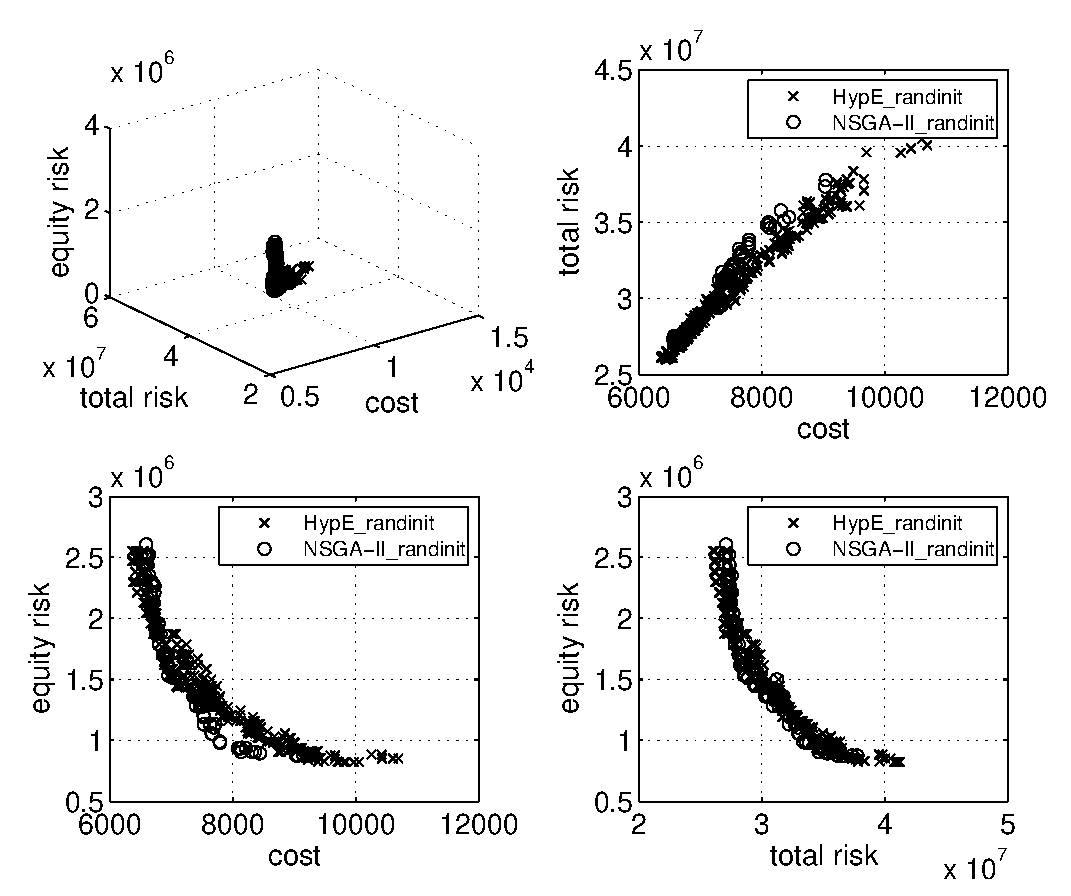
\includegraphics[width=\columnwidth]{../experiments/randVsCost/allsolutions.eps}%
	\caption{\label{fig:allsolutions} Comparison between the random initialization (circles) and the cost-optimal one (crosses). Shown are the populations of 10 independent HypE runs after 1000 generations for all three objectives (top left) and each combination of two objectives.}
\end{figure}

\begin{figure}%
	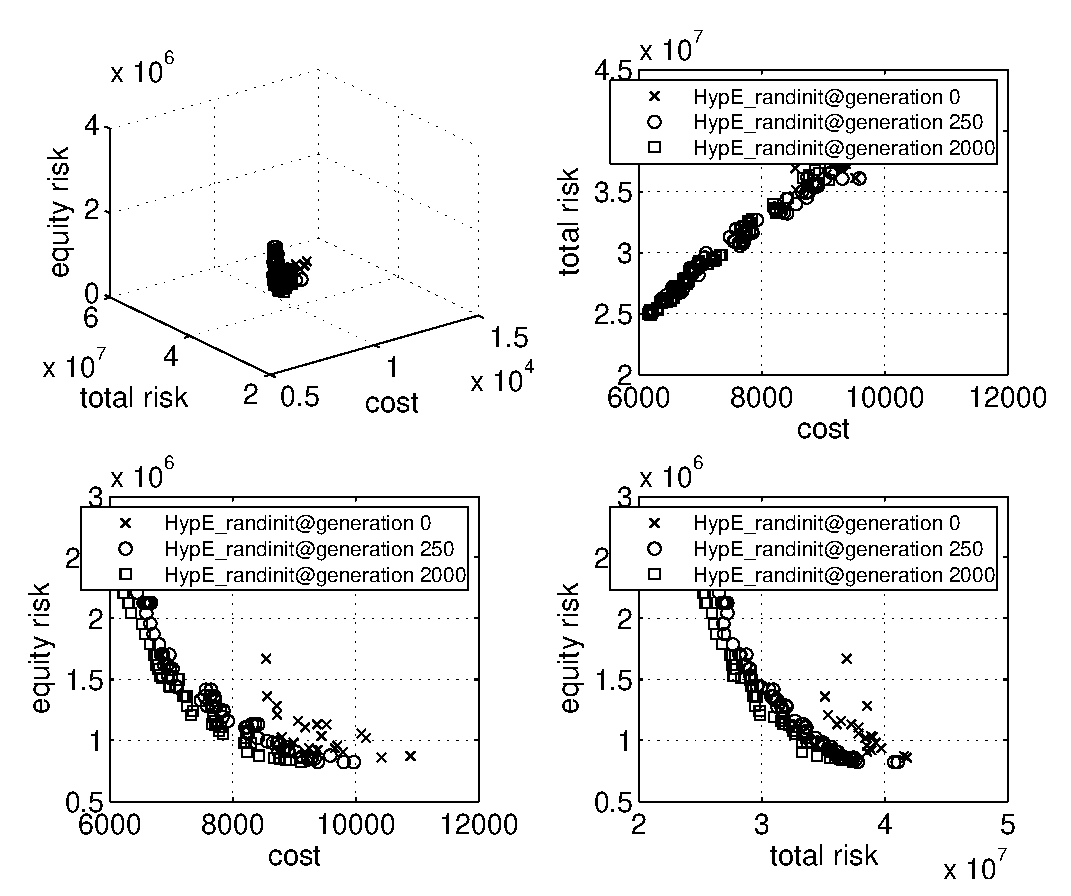
\includegraphics[width=\columnwidth]{../experiments/randVsCost/onlynondominated.eps}%
	\caption{\label{fig:onlynondominated} Comparison between the random initialization (circles) and the cost-optimal one (crosses). Shown are only the non-dominated solutions in the final populations of 10 independent HypE runs after 1000 generations.}
\end{figure}


\subsection{Comparison With An Exact Algorithm for the Two Linear Objectives}
\TODO{add plots and describe what we compare (efficient cost/risk paths multiplied by the number of trucks); result: EA is better}

\subsection{Changing the Population Size}
In a second experiment, we show that changing the population size of the algorithm in standard ranges does not change the algorithm outcome drastically. To this end, Fig.~\ref{fig:popsizes} shows the nondominated solutions of 10 independent runs after 100,000 function evaluations for three different versions of HypE where the population size changes from 50 over 100 to 200 on the largest instance lazio\_4\_1 with 4 commodities. From the visual inspection of the resulting solutions, we cannot make a statement about which population size to favour. When comparing the hypervolume values of the resulting populations, however, an effect is visible. Figure~\ref{fig:algoComparison} shows the corresponding box plots of the hypervolume values and one-sided Wilcoxon rank sum tests on the populations' hypervolume indicator values reveil statistical significant differences between two of the three possible algorithm pairs. With a $p$-value of $0.02163$, the null hypothesis of no differences between a population size of 50 and a population size of 100 has to be rejected in favor of stating that the algorithm variant with population size 50 is superior to the one with population size 100. For the comparison between population size 50 and population size 200, the $p$-value equals $0.0144$ with the population size 50 being better whereas the comparison between population size 100 and population size 200 does not reveal a statistical difference (the $p$-values of the one-sided Wilcoxon tests are $0.2179$ and $0.8035$ respectively). 

Although these results indicate that smaller population sizes might be always favorable, this is not the case as additional experiments with a population size of 25 show (see the box plot in Fig.~\ref{fig:algoComparison}). The Wilcoxon rank sum test comparing population sizes 25 and 50 results in a $p$-value of $0.004465$ whereas the other comparisons are not statistically significantly different. To conclude, among the tested population sizes, 50 seems to be the best choice for budgets around 100,000 function evaluations. Also with longer runs, we recommend to keep the population size of the algorithm around 50 as the HypE implementation in PISA becomes too costly if the population size is much larger. Ten runs with 2000 iterations and population size 200, for example, need already around 20 hours to complete on an Intel Core2 Duo with 2.8GHz.

\begin{figure}%
	\centering
	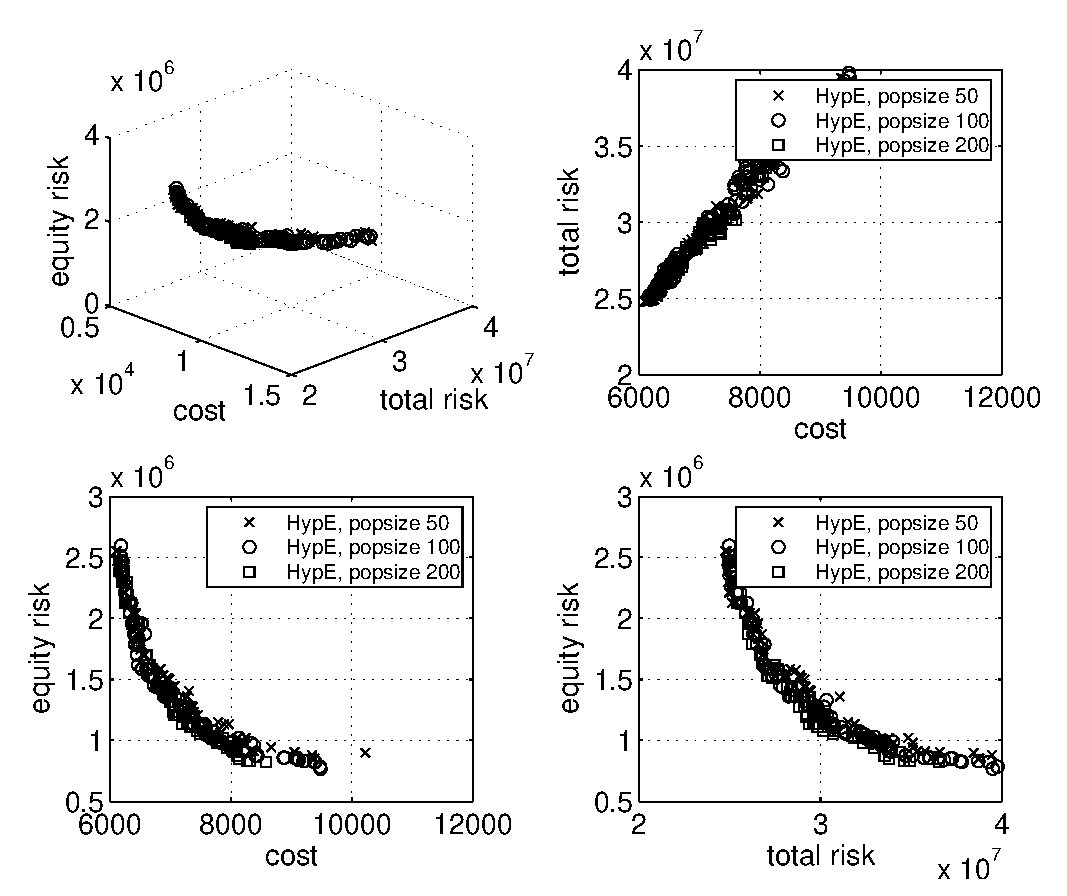
\includegraphics[width=0.8\columnwidth]{../experiments/randVsCost/diffPopsizes}%
	\caption{\label{fig:popsizes} Nondominated solutions of 10 independent runs after 100,000 function evaluations for HypE with a population size of 50 ($\times$), 100 ($\circ$), and 200 ($\square$) respectively.}
\end{figure}

\begin{figure}%
	\centering
	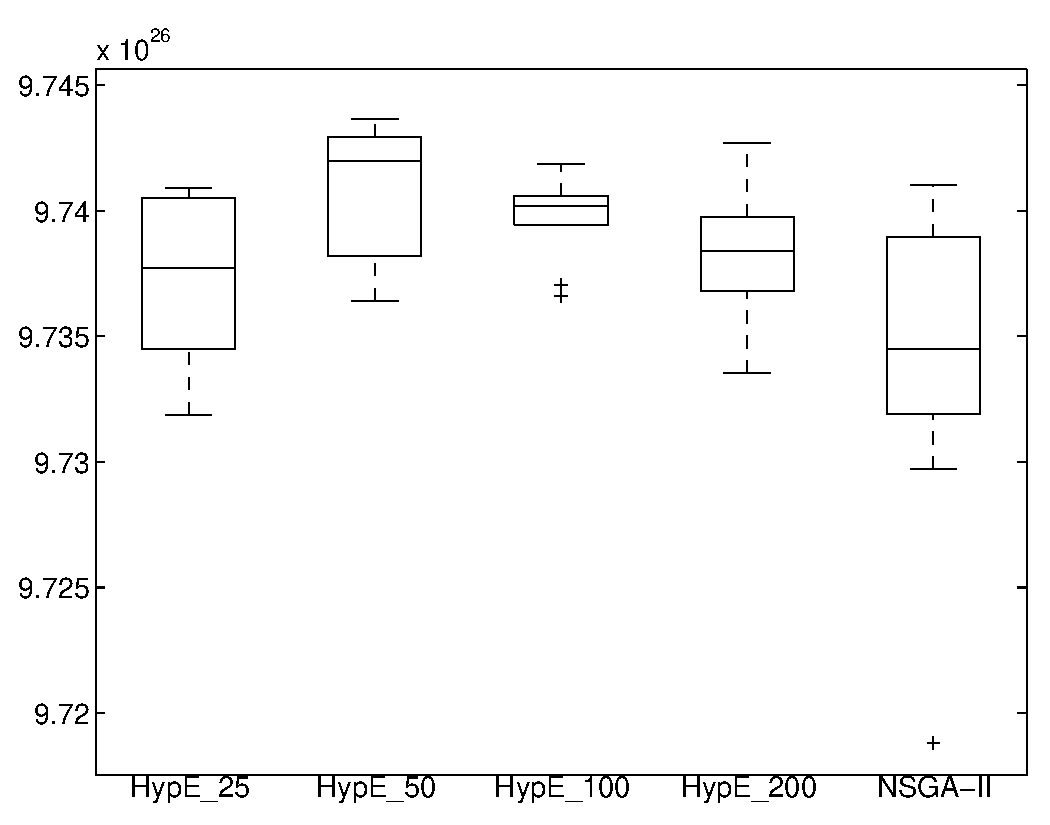
\includegraphics[width=0.5\columnwidth]{../experiments/randVsCost/hypervolumes/algoComparison}%
	\caption{\label{fig:algoComparison} Boxplots of the hypervolume values of 10 independent runs after 100,000 function evaluations of HypE with a population size of 25, 50, 100, and 200, as well as for NSGA-II.}
\end{figure}

\subsection{Changing the Environmental Selection}
With a last experiment, we show the influence of the algorithm's environmental selection scheme on the performance and in particular how this can be used to steer the search towards specific regions of the Pareto front.
\TODO{write}


\subsection{The Feasibility of the EMO Approach}
\begin{itemize}
	\item of course no guarantee that the solutions are Pareto-optimal
	\item however, in reasonable time (e.g. ??hrs for 10 runs with 1000 generations each) results with several non-dominated solutions the decision maker can interpret and with which she can get an idea about the trade-offs between the objectives
	\item if DM wants good results fast, cost-efficient initialization is favourable, otherwise, random initialization gives better spread of the solutions
	\item if needed, approach can be combined easily with preference articulation techniques such as the weighted hypervolume indicator which allows to steer the search towards user-defined regions of the objective space (show 1 plot with W-HypE).
	\item approach is very general and can easily deal with slightly modified problems: e.g. different truck loads (only the objective function code needs to be changed)
	\item it needs to be mentioned that for the tested instances with 311 nodes and 441 arcs, the variation operator of the evolutionary algorithm was able to construct the shortest paths from source to destination in some of the runs for some of the truck paths within the first 100,000 function evaluations. This corresponds to performing random walks of lengths around 20 nodes.
\end{itemize}


%%%%%%%%%%%%%%%%%%%%%%%%%%%%%%%%%%%%%%%%%%%%%%%%%%%%%%%%%%%%%%%%%%%%%%%%%
\section{Conclusions} \label{S_FW}
%%%%%%%%%%%%%%%%%%%%%%%%%%%%%%%%%%%%%%%%%%%%%%%%%%%%%%%%%%%%%%%%%%%%%%%%%
The transportation of hazmats is an important optimization problem in the field of sustainable development and in particular the equitable distribution of risks is of high interest. Within this study, we formalize this transportation problem as the minimization of three objectives and propose to use an evolutionary algorithm to cope with the non-linear equity risk objective.

The third objective function of our problem can be rewritten by minimizing the additional variable $z$ as third objective and adding the constraints $\forall q \in Q: z \geq \sum_{c \in C} \sum_{(i,j) \in A} r_{ij}^{cq} f_{ij}^c$. Although this equivalent formulation makes the problem linear (with additional linear constraints), classical algorithms are expected to have difficulties with this formulation as well and our algorithm is supposed to be more efficient in the current formulation due to the fewer number of constraints. Note that, for the moment, the proposed EMO algorithm exists on paper only and an actual implementation has to prove in the future which additional algorithm components (such as problem-specific initialization, recombination operators, or other exact optimization (sub-)procedures) are necessary to generate solutions of sufficient quality and whether adaptively changing the number and capacity of trucks is beneficial.


In future work, one might want to look further into adding (simple) heuristics within the evoluionary algorithm in order to improve the algorithm. For example, one can observe that the solutions produced by the algorithm sometimes uses one and the same arc within a truck path, hence introducing cylces. With the three objectives cost, total and equity risk, such cycles can be easily prevented within the variation operator which might eventually result in a faster convergence of the algorithm to the Pareto front.




% The transportation of hazmats is an important optimization problem in the field of sustainable development and in particular the equitable distribution of risks is of high interest. 

% In this study, we formalize transportation of hazmats problem as the minimization of three objectives and propose to use an evolutionary algorithm since many exact optimization procedures have difficulties with the non-linear equity risk objective. Note that our problem formulation can be rewritten by minimizing the additional variable $z$ as third objective and adding the constraints $\forall q \in Q: z \geq \sum_{c \in C} \sum_{(i,j) \in A} r_{ij}^{cq} f_{ij}^c$ \COMMENTD{this has to be adapted according to the new problem formulation}. Although this equivalent formulation makes the problem linear (with additional non-linear constraints), classical algorithms are expected to have difficulties with this formulation as well and the EMO algorithm is supposed to be more efficient in the current formulation due to the fewer number of constraints.
% 
% Note also that, for the moment, the proposed EMO algorithm only exists as a gedankenexperiment and an actual implementation has to prove in the future which additional algorithm components (such as problem-specific initialization, recombination operators, or other exact optimization (sub-)procedures) are necessary to improve the quality of the found solutions to a sufficient level.


\section{Acknowledgments}
The authors would like to thank Stefano Giordani for providing us with the instances of the Lazio network. Moreover, Dimo Brockhoff would like to acknowledge support from the CNRS-Microsoft chair "`Optimization for Sustainable Development"' during his time at Ecole Polytechnique, Palaiseau, France.


% 
 \bibliographystyle{plainnat}
 \footnotesize
% \bibliography{hazmat}

\begin{thebibliography}{00}
% \providecommand{\natexlab}[1]{#1}
% \providecommand{\url}[1]{\texttt{#1}}
% \expandafter\ifx\csname urlstyle\endcsname\relax
%   \providecommand{\doi}[1]{doi: #1}\else
%   \providecommand{\doi}{doi: \begingroup \urlstyle{rm}\Url}\fi

\bibitem[Akgun et~al.(2003)Akgun, Erkut, and Batta]{AKG02}
V. Akgun, E. Erkut and R. Batta, 
On finding dissimilar paths, 
European Journal of Operational Research 121(2):232-246, 2000.

\bibitem[Bader and Zitzler(2011)]{bz2011a}
J.~Bader and E.~Zitzler.
\newblock Hype: An algorithm for fast hypervolume-based many-objective
  optimization.
\newblock \emph{Evolutionary Computation}, 19\penalty0 (1):\penalty0 45�--76,
  2011.

\bibitem[Bleuler et~al.(2003)Bleuler, Laumanns, Thiele, and Zitzler]{bltz2003a}
S.~Bleuler, M.~Laumanns, L.~Thiele, and E.~Zitzler.
\newblock PISA---a platform and programming language independent interface for
  search algorithms.
\newblock In \emph{Evolutionary
  Multi-Criterion Optimization {(EMO~2003)}}, pages
  494--508, 2003. Springer.

\bibitem[Caramia et~al.(2008)Caramia and Dell'Omo]{CAR08}
M. Caramia and P. Dell'Olmo, 
Multiobjective management in freight logistics: increasing capacity, service level and safety with optimization algorithms,
Springer London Ltd, 2008.

\bibitem[{Coello Coello} et~al.(2007){Coello Coello}, {Lamont}, and {Van
  Veldhuizen}]{cvl2007a}
C.~A. {Coello Coello}, G.~B. {Lamont}, and D.~A. {Van Veldhuizen}.
\newblock \emph{Evolutionary Algorithms for Solving Multi-Objective Problems}.
\newblock Springer, 2007.

\bibitem[Deb(2001)]{deb2001a}
K.~Deb.
\newblock \emph{Multi-Objective Optimization Using Evolutionary Algorithms}.
\newblock Wiley, Chichester, UK, 2001.

\bibitem[Horoba(2009)]{horo2009a}
C.~Horoba.
\newblock Analysis of a simple evolutionary algorithm for the multiobjective
  shortest path problem.
\newblock In \emph{Foundations of Genetic Algorithms {(FOGA 2009)}}, pages
  113--120. ACM, 2009. 

\bibitem[bianco(2009)]{bianco09}
L. Bianco and M. Caramia and S. Giordani.
\newblock A bilevel flow model for hazmat transportation network design.
\newblock Transportation research. Part C, Emerging technologies, 17(2):175--196, 2009.



% \bibitem{GOP90b}
% R. Gopalan, K.S. Kolluri, R. Batta and M.H. Karwan, 
% Modeling equity of risk in the transportation of hazardous materials, 
% Operations Research, 38(6):961-973, 1990.
% 
% \bibitem{KUB97}
% M. Kuby, X. Zhongyi and X. Xiaodong, 
% A minimax method for finding the $k$ best differentiated paths, 
% Geographical Analysis 29(4):298-313, 1997.

% \bibitem{LOM93}
% K. Lombard and R.L. Church, 
% The gateway shortest path problem: Generating alternative routes for a corridor location problem, 
% Geographical Systems, 1:25-45, 1993.

\end{thebibliography}


\end{document}

%%
%% End of file `elsarticle-template-1a-num.tex'.
